\documentclass{article}
\usepackage{tikz}
\usepackage{makecell}
\usepackage{nicefrac}
\usetikzlibrary{decorations.markings}

\begin{document}
    \begin{tabular}{|c|c|c|c|}
        \hline
        State & Amplitude & Phase & Ellipse \\ 
        \Xhline{3\arrayrulewidth}
        LHP & $E_{0y}=0$ & $0$ &  \raisebox{3pt}{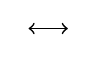
\begin{tikzpicture} \draw[<->, semithick] (0,0) -- (0.5,0); \end{tikzpicture}} \\
        \hline
        LVP & $E_{0x}=0$ & 0 & \raisebox{-4pt}{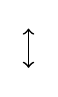
\begin{tikzpicture} \draw[<->, semithick] (0,0) -- (0,0.5); \end{tikzpicture}} \\
        \Xhline{2\arrayrulewidth}
        $L_{+45}P$ & $E_{0x}=E_{0y}$ & 0 & \raisebox{-3pt}{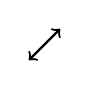
\begin{tikzpicture}
        \draw
        [<->, thick] 
        (0,0) -- (0.4,0.4);
        \end{tikzpicture}}
        \\
        \hline
        $L_{-45}P$ & $E_{0x}=E_{0y}$ & $\pi$ & \raisebox{-3pt}{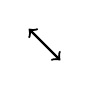
\begin{tikzpicture}
        \draw
        [<->, thick] 
        (0,0) -- (-0.4,0.4);
        \end{tikzpicture}} \\
        \Xhline{2\arrayrulewidth}
        RCP & $E_{0x}=E_{0y}$ & $\nicefrac{\pi}{2}$ & 
        \raisebox{-4pt}{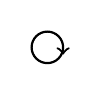
\begin{tikzpicture}
        \useasboundingbox (-0.25,-0.25) rectangle (0.25,0.25);
        \draw
        [thick, decoration={markings, mark=at position 0 with {\arrow{<}}}, postaction={decorate}]
        (0,0) circle (0.2);
        \end{tikzpicture}} \\
        \hline
        LCP & $E_{0x}=E_{0y}$ & $-\nicefrac{\pi}{2}$ & 
        \raisebox{-4pt}{
\begin{tikzpicture}
        \useasboundingbox (-0.25,-0.25) rectangle (0.25,0.25);
        \draw
        [thick, decoration={markings, mark=at position 0 with {\arrow{>}}}, postaction={decorate}] (0,0) circle (0.2);
        \end{tikzpicture}} \\
        \hline
    \end{tabular}
\end{document}
